It was already discussed in \cref{sec: autoquad} 
how the flight control of modern UAV is structured. 
Since this work aims at using reinforcement learning to learn a robust control of a quadrocopter, the explained does not fit this structure. 
\cref{fig:autoquad} shows the use of a mission goal controller that shows some distant resemblance to the implemented intelligent agent. 
In Contrast, it does not output a desired attitude to achieve the defined goal, but directly outputs actions that are more or less the motor values. 
As a consequence there is no need for a classic Attitude Control but a need of controlling the motor signals to match the actions.
This chapter proposes a flight control concept with the use of an intelligent agent. 
Also, it provides a general concept of the implementation in order to get a wider view at the different implemented classes, tools and scripts.\\
\newline
At each timestep $t$ the agent receives a mission goal $\overrightarrow{g}=(g_x, g_y, g_z)$ 
and a normalization of the position/state estimation $p=(p_x, p_y, p_z, \Theta, \phi, \psi, \dot{p_x}, \dot{p_y}, \dot{p_z}, \dot{\Theta}, \dot{\phi}, \dot{\psi})$
 and outputs a 4-tupel of actions $a = (a_0, a_1, a_2, a_3)$ with each $a_i \in [-1,1], i \in [0,1,2,3]$. This can be denormalized to a signal $S_N$. 
 On a real UAV this would be most likely a pwm signal. With the use of a speed controller the signal is held at the specific value. 
 With the use of the motors and props there is a thrust $\tilde{f}$ and a corresponding state transition that can be observed by the sensors. 
 These sensor values $\sigma$ can be used in order to estimate the position and normalize it to the range $[-1,1]$. 
 This concept is visualized in \cref{fig:conceptAuto}.

\begin{figure}[htp]
	\centering
	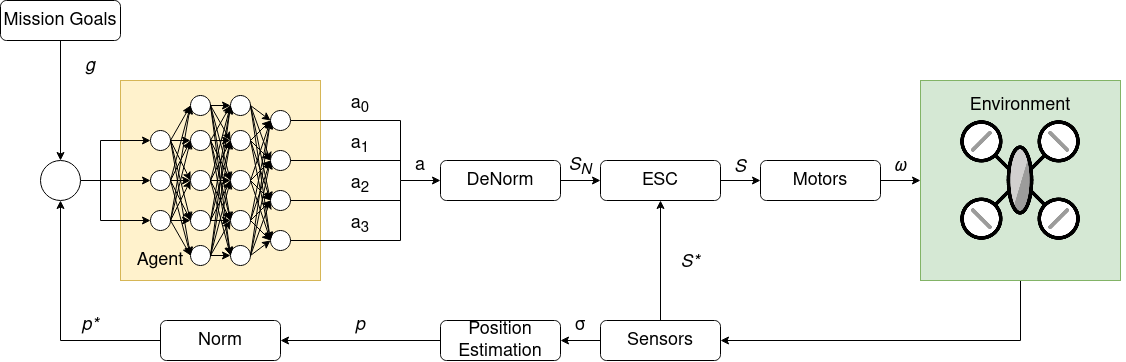
\includegraphics[width= 0.9 \linewidth]{figures/conceptAuto.png}
	\caption{Proposed Concept of autonomous flight control with the use of an intelligent agent implemented with the use of a NN. 
	The output of the NN is denormalized in order to translate them to motor signals. 
	With the use of the sensors and position estimation the input for the next control step are calculated.}
	\label{fig:conceptAuto}
\end{figure}

\newpage

